\documentclass[letterpaper]{article}

% if you need to pass options to natbib, use, e.g.:
% \PassOptionsToPackage{numbers, compress}{natbib}
% before loading nips_2017

% ready for submission
\usepackage[final]{nips_2017}

\usepackage[utf8]{inputenc} % allow utf-8 input
\usepackage[T1]{fontenc}    % use 8-bit T1 fonts
\usepackage{hyperref}       % hyperlinks
\usepackage{url}            % simple URL typesetting
\usepackage{booktabs}       % professional-quality tables
\usepackage{amsmath}
\usepackage{amsfonts}       % blackboard math symbols
\usepackage{graphicx}
\usepackage{lmodern}
\usepackage{nicefrac}       % compact symbols for 1/2, etc.
\usepackage{microtype}      % microtypography

\title{Multitask Object Detection with Dropout and Neural Code Metric Learning}

\author{
  Philip Pham \\
  University of Washington \\
  \href{pmp10@uw.edu}{\texttt{pmp10@uw.edu}} \\
}

\begin{document}

\maketitle

\begin{abstract}
  Using techniques and theory discussed in CSE 547, we try to detect objects in
  images with classification model and retrieve images with metric learning. The
  object detection task was seen as multi-label classification problem. Using
  multitask learning and dropout regularization, a neural network was trained to
  detect objects in patches. The last hidden layer of this network was used for
  neural code metric learning. Neighbors were retrieved with a ball tree.
\end{abstract}

\section{Introduction}

The COCO dataset consists of 330,000 images. Each image is annotated with
bounding boxes which contain objects belonging to one of 80 categories
\citep{coco}. Using this dataset, I explored several techniques covered in CSE
547 including neural networks, non-convex optimization, metric learning, and
nearest neighbor methods.

My objectives where:
\begin{itemize}
\item (\emph{object detection}) given an image, extract patches that contain an
  object and classify the object;
\item and (\emph{metric learning}) define a distance metric that compares
  patches such that patches of the same categories are close together, and
  patches of different categories are far apart.
\end{itemize}

In particular, I explored different neural network architecures with various
learning strategies before settling on a multi-layer perceptron model with
dropout. For the metric learning, I attemped to use neural codes
\citep{neural_codes}. Then, the nearest neighbor search is done using a ball
tree.

\section{Methods and Materials}

For object detection, regions were proposed with selective search
\citep{selective_search}. Features for each image were given based on
\cite{fast_rnn}. A fixed length feature vector was extracted for each patch
using pooling \citep{pooling}. For an example of region proposals by selective
search, see Figure \ref{fig:coco_selective_search}.

\begin{figure}
  \centering
  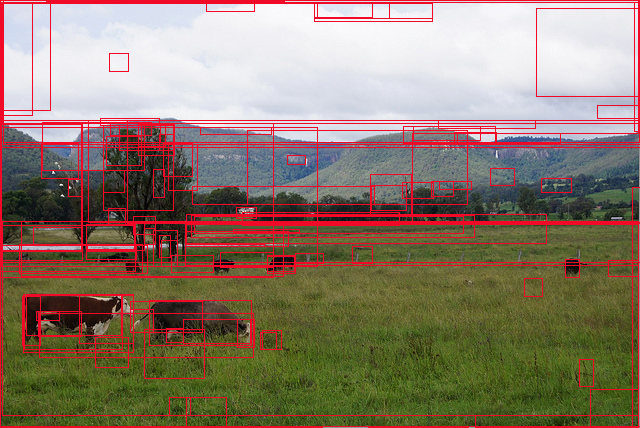
\includegraphics[width=0.7\textwidth]{../hw3/bounding_box_sample.png}
  \caption{Top 128 region proposals by selective search for COCO image 364814.}
  \label{fig:coco_selective_search}
\end{figure}

Using annotations provided by the COCO API, training, validation, and test
datasets were constructed from the patches from the region proposoals with
intersection over union (IoU) over 0.5 with a bouding box from an
annotation. That patch was then labeled with the categories from the annotated
bounding box.

To simplify the problem, we were provided with two subsets of the COCO dataset:
\texttt{tiny} and \texttt{small}. The \texttt{small} dataset was used. In this
dataset, for each image a $256 \times 13 \times 13$ array of features was
provided from a convolutional neural network like the one described in
\cite{fast_rnn}.

The training set consisted of 375,453 patches from 10,000 images. The test set
was 74,276 patches from 2,000 images, and the validation set was 75,620 patches
from 2,000 images. Each patch had 11,776 features. From here, the problem can be
seen as a multi-label classification problem. Models were trained with PyTorch
\citep{pytorch}.

The neural codes for the metric learning were extracted from the last hidden
layer of the multi-layer perceptron used for object detection. To find nearest
neighbors, a ball tree from \texttt{sklearn} was used \citep{scikit-learn}.

\section{Results}

The best unweighted mean average precision on the test set was
0.254112\unskip. With the
learned metric, the nearest neighbor was of the same category 24\% of the
time.

\subsection{Object Detection}

The multi-layer perceptron with dropout performed best. It consisted of two
hidden layers with 1,024 and 256 units, respectively. At each layer, dropout
with $p = 0.5$ and ReLu activation functions were used.

\subsubsection{Models}

Three types of models were trained for object detection. You can see the
results in Table \ref{tab:model_comparison}. $L2$-regularization parameters
and the number of hidden units were tuned to produce the smallest loss on the
validation dataset. The idea behind using an MLP is that it enables
weight-sharing in the hidden units. One might imagine certain animals or
vehicles have common features that the model could learn together.

\begin{table}[h]
  \centering
  \begin{tabular}{lrr}
\toprule
Model &  Average Precision Score &      Loss \\
\midrule
Linear   &                 0.1750 &  0.1946 \\
  2-layer MLP &                 0.2198 &  0.1824 \\
  MLP with Dropout & 0.2351 & 0.1807 \\
\bottomrule
\end{tabular}
  
  \caption{Metrics are computed against the validation dataset.}
  \label{tab:model_comparison}    
\end{table}

To use multitask learning, multi-label cross entropy was used for the loss
function. The $L2$-regularization parameter $\lambda$ by looking at the
difference between validation and training loss across various training
runs. While there were large differences, regularization was
increased. Eventually, validation loss stopped improving. See Figure
\ref{fig:training_loss} for a plot of training and validation loss as function
of training steps. See Figure \ref{fig:training_average_precision_score} for a
similar plot regarding the average precision score computed with macro
averaging.

\begin{figure}
  \centering
  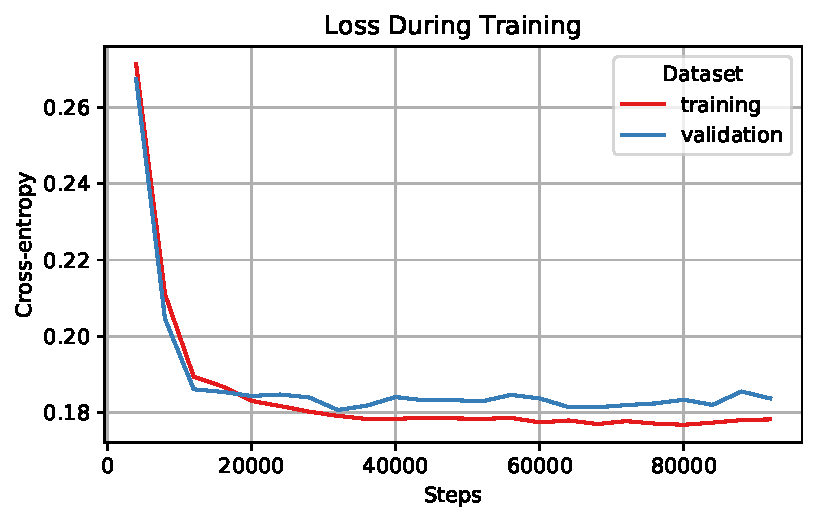
\includegraphics{object_detection/training_loss.pdf}
  \caption{Loss was calculated after every 4,000 steps.}
  \label{fig:training_loss}
\end{figure}

\begin{figure}
  \centering
  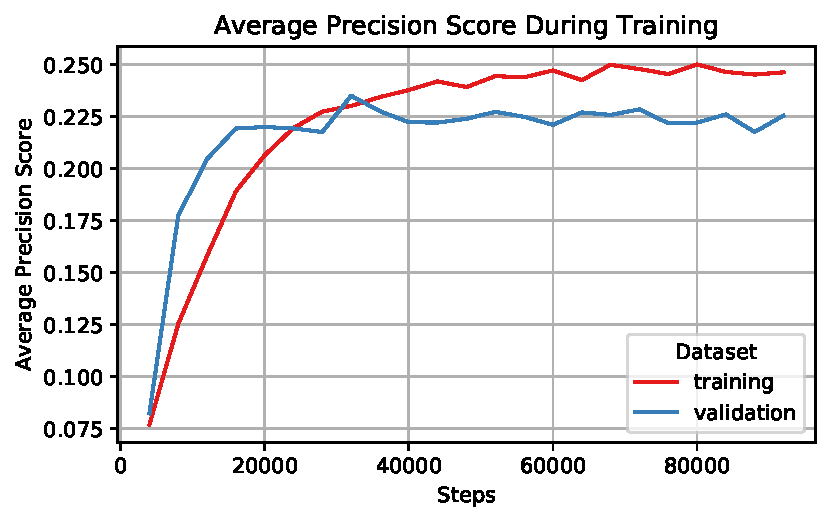
\includegraphics{object_detection/training_average_precision_score.pdf}
  \caption{Mean average precision score was calculated after every 4,000 steps
    with a macro averaging strategy across categories.}
  \label{fig:training_average_precision_score}
\end{figure}

To obtain a further improvement, dropout regularization was applied. Dropout is
a form of regularization that randomly zeroes outs a hidden unit during training
\citep{dropout}. Intuitively, this prevents the network from seeing the same
examples and avoids memorizing the training data.

\subsubsection{Model Evaluation}

When evaluated against the test dataset, the mean average precision was
0.254112taken as
unweighted average over the classes.

If one looks at the class breakdown in Table
\ref{tab:average_precision_score_by_class}, one sees that have under-represented
classes tend to have lower scores, for getting them wrong has less impact on
loss.

\begin{table}
  \centering
  \begin{tabular}{lrrr}
\toprule
      Label &  Training Observations &  Test Observations &  Average Precision Score \\
\midrule
    bicycle &                   9950 &               1847 &                 0.027483 \\
        car &                  56694 &              11010 &                 0.362490 \\
 motorcycle &                  13163 &               2757 &                 0.040598 \\
   airplane &                  15830 &               2529 &                 0.077730 \\
        bus &                  16103 &               2985 &                 0.087326 \\
      train &                   4568 &                873 &                 0.040963 \\
      truck &                  29670 &               6045 &                 0.117114 \\
       boat &                  15037 &               3179 &                 0.057605 \\
       bird &                  28911 &               6232 &                 0.314083 \\
        cat &                  12070 &               2778 &                 0.500823 \\
        dog &                  15957 &               2629 &                 0.240831 \\
      horse &                  22997 &               4966 &                 0.272576 \\
      sheep &                  34010 &               6046 &                 0.421672 \\
        cow &                  34359 &               7271 &                 0.318933 \\
   elephant &                  23508 &               3972 &                 0.454776 \\
       bear &                   3827 &                578 &                 0.018140 \\
      zebra &                  25923 &               5720 &                 0.578105 \\
    giraffe &                  19805 &               4243 &                 0.642767 \\
\bottomrule
\end{tabular}

  \caption{Class breakdown of average precision score.}
  \label{tab:average_precision_score_by_class}
\end{table}

\subsection{Metric Learning}

\cite{neural_codes} and \cite{imagenet} suggest that the top layer of a network
may summarize an image, so I thought to try extract that layer to use as an
embedding. Let $f$ be my neural network. We can write $f = g \circ h$, where $h$
takes the patch features and outputs 256-dimensional vector that forms the last
hidden layer. Then, the distance metric for two patches $P$ and $P^\prime$ is
$d\left(P,P^\prime\right) = \left\lVert h\left(P\right) -
  h\left(P^\prime\right)\right\rVert_2$.

Once each patch was embedded into $\mathbb{R}^{256}$, a ball tree was used to
enable fast nearest neighbor retrieval. If one fixes $K \in \mathbb{N}$, one has
a classifier for category $C$ by taking the percentage of the $K$ nearest
neighbors that belong to category $C$.

In light of this, we have that the average precision score for a class $C$ is
\begin{equation}
  \frac{1}{\text{\# of patches of class $C$}}
  \sum_{\{P~:~\text{P has label $C$}\}}\frac{\text{\# of $K$ nearest neighbors of $P$ category $C$}}{K}.
\end{equation}
We take the unweighted average of this across categories at different values of
$K$ to obtain Figure \ref{fig:metric_average_precision_score}.

\begin{figure}[h]
  \centering
  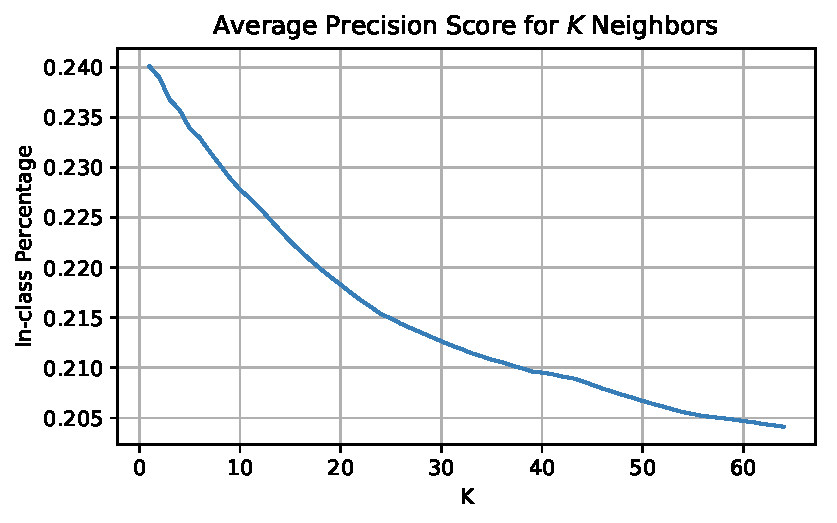
\includegraphics{metric_learning/metric_average_precision_score.pdf}
  \caption{For $K$ up to 64, the average precision score was calculated.}
  \label{fig:metric_average_precision_score}
\end{figure}

The nearest neighbor is most likely to be of the same category. Increasing $K$
does not seem to help as the additional neighbors do not appear to more likely
to be of the correct category.

Table \ref{tab:metric_learning_class} shows these results broken down by
class. The nearest neighbor is of the same category about a quarter of time
overall, but varies for some categories. These results roughly mirror those in
Table \ref{tab:average_precision_score_by_class} with categories that occur more
frequently in the training data doing better. In some rare instances, like
\texttt{bird}, \texttt{cat}, \texttt{dog}, and \texttt{cow}, the next few
neighbors are more likely to be of the same category, too, so average precision
score for these classes increases with $K$ to a point.

\begin{table}
  \centering
  \begin{tabular}{lrrrrr}
\toprule
            & \multicolumn{5}{l}{Number of Neighbors} \\
      Label &               K = 1 &     K = 3 &     K = 5 &    K = 10 &    K = 15 \\
\midrule
    bicycle &            0.042793 &  0.046547 &  0.044257 &  0.043187 &  0.043919 \\
        car &            0.314220 &  0.309779 &  0.307115 &  0.291930 &  0.287312 \\
 motorcycle &            0.051215 &  0.049844 &  0.049047 &  0.046280 &  0.045134 \\
   airplane &            0.061684 &  0.063662 &  0.062554 &  0.058600 &  0.058521 \\
        bus &            0.106321 &  0.100110 &  0.094995 &  0.095543 &  0.091804 \\
      train &            0.044499 &  0.040379 &  0.037824 &  0.034981 &  0.037165 \\
      truck &            0.147673 &  0.134968 &  0.126489 &  0.121318 &  0.120335 \\
       boat &            0.098957 &  0.088207 &  0.083908 &  0.075624 &  0.075603 \\
       bird &            0.208440 &  0.216303 &  0.214121 &  0.208521 &  0.197925 \\
        cat &            0.287394 &  0.301850 &  0.301360 &  0.302536 &  0.289599 \\
        dog &            0.289124 &  0.296166 &  0.284507 &  0.271753 &  0.266249 \\
      horse &            0.242839 &  0.223252 &  0.217355 &  0.206529 &  0.198905 \\
      sheep &            0.296334 &  0.295381 &  0.294618 &  0.289876 &  0.291456 \\
        cow &            0.285961 &  0.286681 &  0.288553 &  0.289590 &  0.279952 \\
   elephant &            0.256494 &  0.251366 &  0.255687 &  0.261892 &  0.267474 \\
       bear &            0.127273 &  0.101818 &  0.097455 &  0.082364 &  0.073576 \\
      zebra &            0.379962 &  0.376348 &  0.370869 &  0.351582 &  0.333310 \\
    giraffe &            0.350071 &  0.340798 &  0.336445 &  0.339981 &  0.335691 \\
\bottomrule
\end{tabular}

  \caption{For each patch, the percentage of neighbors belonging to the
    same one was calculated and then averaged.}
  \label{tab:metric_learning_class}
\end{table}

\section{Discussion}

My model does not perform nearly as well as other models in the literature. For
example, \cite{benchmark} achieve a baseline mean average precision score of
0.415 with VGG-16. Using residual networks (ResNet-101), they achieved
0.484. With further refinements around input processing, they achieve 0.538.

Some possible improvements to improve object detection are harnessing more of
the COCO dataset and exploring more complicated network architecures like
convolutions and residual networks. These techniques would require more compute
and memory.

My neural network currently generates the metric without any knowledge that the
last hidden layer will be used as a metric. One promising way to incorporate
this knowledge is a \emph{siamese architecture} \citep{siamese}. This
architecure shares the weights between two identical networks. Each network
takes a patch as input and our loss function is constructed such that small
differences between patches of the same category and large differences between
patches of different categories are favored.

It may be worth incorporating this loss function into a multitask learning
framework, so weights are shared for the object detection model, too. One can
image there are features that could be learned that are both useful for both
retrieving similar images and classifying patches.

\bibliographystyle{chicago}
\bibliography{references}

\end{document}
